\clearpage
\section{Organiser les données}\label{sec:organiser-donnees}

On a vu dans la première partie de ce chapitre (\cref{sec:sorties-simfeodal}) que les données produites par SimFeodal étaient nombreuses, diverses et massives.
Contrairement à des modèles de simulations plus \og KISS \fg{}, par exemple les \og modèles-jouets\fg{} courants en Sciences Humaines et Sociales (\hl{ref Schelling/Sakoda, SugarScape, Prey-Predator, }), SimFeodal fait ainsi interagir de nombreux types d'agents, chacun doté de sorties spécifiques. Ces modèles sont le plus souvent évalués \og en direct\fg{}, les indicateurs présents dans l'interface des plate-forme de simulations suffisant à leur compréhension.
La démarche suivie pour l'évaluation de SimFeodal repose sur des indicateurs visuels, qui doivent être examinés \textit{a posteriori} de leur production (\cref{subsec:observation-a-posteriori}), et l'évaluation du modèle ne peut être réalisée qu'en s'appuyant sur une part importante de ces sorties.

Dans les modèles plus complexes utilisés en géographie (\hl{SimPop, MobiSim, SimPopLocal, MARIUS}), les données peuvent être plus massives (que ce soit intrinsèque au modèle (MobiSim) ou à sa méthode d'exploration (SimPopLocal)), mais leur structuration, souvent mono-agent, reste simple.

Pour SimFeodal, où les indicateurs s'appuient parfois sur des requêtes croisant plusieurs types d'agents, la question de la structuration de ces données revêt une importance cruciale.
Sans structuration adéquate, l'acquisition, l'archivage, l'interrogation ou encore la sauvegarde des données générées par le modèle ne peuvent être garantis, et encore moins de manière efficace.

Le choix d'une méthode d'organisation des données en sortie de simulations ne relève donc pas ici d'une quelconque coquetterie technique, mais, au contraire, conditionne et contraint fortement aussi bien les modalités de création des indicateurs que les possibilités de la plate-forme d'exploration de les afficher de manière interactive.

	\subsection{Assurer la capacité d'interrogation des données}\label{subsec:capacite-interrogation}

	Avant de se soucier du \og schéma\fg{} de la base de données\footnote{
		On utilise souvent le terme de \og schéma\fg{} pour désigner la version implémentée, dans un SGBD spécifique, du Modèle Conceptuel de Données (MCD). Contrairement au MCD, qui donne une version conceptuelle et générique d'une base de données, le schéma est donc tributaire du SGBD dans lequel il est intégré.
	}, du choix du Système de Gestion de Base de Données (SGBD), ou encore des performances de ce dernier, il convient de se fixer sur la manière dont on souhaite entreposer les données.

	De la myriade de fichiers issus de tableurs organisés dans une multitude de dossiers spécifiques à l'entrepôt de données décentralisé orienté documents, en passant par les traditionnelles bases de données relationnelles, les possibilités de stockage et d'organisation des données issues de simulations sont ainsi innombrables.

	Qui plus est, dans le but de générer et d'afficher des indicateurs de sorties de simulation \og à la volée \fg{}, la méthode d'interrogation (ou de \og requêtage \fg{}) des données stockées est un choix majeur, qui doit à ce titre précéder les autres.

	Dans le cadre des données issues de SimFeodal, en vue de leur mobilisation dans SimEDB, nous avons ainsi eu à sélectionner quelques SGBD candidats parmi foule de solution possibles.
	Afin de guider ce choix, trois critères ont été définies, et forment, selon une hiérarchie propre à leur ordre, un ensemble de filtre ayant permis la réduction des SGBD possibles à un nombre appréhendable.
	Ces critères, dont l'énonciation guidera cette partie, sont ainsi (1) l'universalité, ou \og agnosticité\fg{}, des SGBD aux outils de requête ; (2) la pérennité et stabilité des solutions disponibles et (3) les performances des SGBD considérés.

		\subsubsection{Interroger de manière universelle et indépendante}

		Lors de la conception d'un outil faisant appel à des données, qui plus est massives, il convient de se positionner tôt sur la manière d'interroger ces données.
		Par interrogation, on entend ici, comme souvent dans le domaine des bases de données, la manière de faire appel, concrètement, aux données, pour en tirer les sous-ensembles, agrégations et autres résultats synthétiques résultant du traitement des données brutes.
		Si l'on considère des données stockées dans un tableur, alors les \og formules \fg{}, les tableaux croisés dynamiques ou encore les graphiques issus du tableur sont des interrogations des données, qui s'expriment dans ce cas via un ensemble de langages, écrits -- les formules, qui font appel à des fonctions spécifiques des tableurs -- ou visuels -- les tableaux croisés dynamiques, construits en faisant glisser des intitulés de colonnes dans un tableau.

			\paragraph*{Stockage distribué ou centralisé}\label{par:stockage-centralise}
			Avant même de s'intéresser aux spécificités de ces langages, un premier choix réside dans le mode de stockage des données qui doivent être mis à disposition d'une plate-forme.
			Doit-on laisser l'utilisateur intégrer lui-même les données, et ainsi, en faire un stockage \og distribué \fg{}, dans le sens où chaque utilisateur de l'application possèderait physiquement une copie locale des données ?
			Ou, au contraire, les données doivent-elles être centralisées, c'est-à-dire enregistrées en une seule copie à laquelle les utilisateurs accèderaient à distance ?
			Pour reprendre l'exemple des tableurs, doit-on privilégier une solution locale -- chacun ayant une copie du fichier tableur et menant ses propres modifications dessus -- ou une approche de type centralisée, par exemple en privilégiant des tableurs collaboratifs en ligne (\textit{Google Docs/Sheets} par exemple) ?

			Habituellement, c'est-à-dire dans une grande majorité d'applications, les données sont stockées localement : cela permet, en particulier, de ne pas dépendre d'une connexion internet pour interroger des données qui seraient hébergées sur internet.
			Dans le cas de SimFeodal, cette solution est rendue difficile, sinon impossible, par la masse de données en sortie de simulations.
			Si chaque utilisateur de SimEDB devait posséder une copie des données, voir plusieurs en cas d'utilisations depuis différents ordinateurs, cela occuperait plusieurs gigaoctets de données à chaque fois.
			De plus, en cas de mise à jour des données, c'est-à-dire d'insertions de nouvelles sorties de simulations, il faudrait distribuer à nouveau l'ensemble du jeu de données, à chaque fois.

			Pour ces raisons, nous avons fait le choix d'un stockage centralisé, sous forme d'une architecture \og client-serveur\fg{}, hébergé sur un serveur internet dédié, ce qui permet à la plate-forme de travailler à chaque fois sur les données les plus à jour, réduit la taille du stockage physique associé, et dispense d'une configuration sur chaque poste utilisateur :
			si le lien entre l'application et les données fonctionne correctement pour un utilisateur, il fonctionnera à l'identique pour tous les autres.
			Ce choix présente un dernier avantage, non négligeable :
			en stockant les données en un seul lieu, c'est-à-dire sur un serveur informatique, on peut faire en sorte de rendre ce serveur aussi performant que possible, et accélérer ainsi l'interrogation des données pour tous les utilisateurs.

			\paragraph*{Interrogation spécifique ou générique}\label{par:interrogation-generique}

			De nombreuses solutions intégrées de gestion de données proposent leurs propres modes d'interaction avec les données, c'est-à-dire un langage spécifique permettant d'interroger les données contenues dans le système\footnote{
				Souvent, cette interrogation se fait par appel à des \textit{API} (\textit{Application Programming Interface}, ou Interface de Programmation Applicative en français) propres aux plate-formes, demandant donc un langage de requête spécifique.
			}.
			Au contraire, les SGBD les plus classiques s'appuient plutôt sur des langages de requêtes aussi standardisés que possibles, afin de faciliter l'adoption de leur propre solution à des utilisateurs d'autres plate-formes.
			La spécificité présente l'avantage de langages plus adaptés aux données manipulées, et donc souvent plus intuitifs dans l'interrogation des spécificités des données.
			De plus, la spécificité permet aussi une optimisation des requêtes, et est donc souvent plus performante que les solutions plus génériques.

			Dans le cas des données de SimFeodal, nous avons préféré privilégier une approche plus générique, faisant appel à des solutions de SGBD plus standardisées.
			La raison tient principalement à une volonté de généricité du stockage des données : au cours des différentes étapes de construction de SimFeodal, les besoins en matières d'interrogation des données ont évolué.
			Cette évolution était prévisible et prévue, et nous avons donc choisi dès le départ d'adopter uniquement des solutions modulaires, garantissant une évolutivité facilitée de la base de données, aussi bien regardant sa structure (enregistrement de nouvelles variables ou de nouveaux agents du modèle) que son contenu (massification des données en sortie au fur et à mesure de l'exploration du modèle).

			De plus, dans la perspective de ce travail de thèse, où l'on cherche à rendre autant les productions aussi reproductibles et génériques que possible, il était indispensable de disposer d'un SGBD aussi standard que possible pour en faciliter l'adoption et l'adaptation à d'autres modèles de simulations par exemple.

			\paragraph*{SQL ou NoSQL}\label{par:sql-nosql}

			Même une fois arrêté sur le choix de ne faire appel qu'à des outils standards pour stocker les données, le nombre de solutions disponibles demeure très important.
			Afin de réduire ce nombre, on peut déjà choisir les grands types de SGBD auxquels faire appel.
			Les SGBD sont ainsi souvent classés selon les grands traits de la méthode dont ils organisent les données.
			Les deux grands types\footnote{
				Il en existe d'autres, comme les SGBD orientés objets (quasiment disparus aujourd'hui), orientés graphes (Neo4j\ldots), les SGBD pensés pour le stockage et l'interrogation d'ontologies (\textit{Triplestores RDF}, interrogeables en langage SPARQL) ou encore les nouveaux SGBD de type \og NewSQL \fg{} (Apache Ignite, CockRoachDB\ldots) pensés pour une parallélisation massive des données. Ces types de SGBD ne correspondent toutefois pas du tout aux besoins identifiés pour SimEDB/SimFeodal, et sont en général dédiés à des problèmes et marchés de niches. Nous ne les décrirons donc pas plus en détail ici.
			} sont les SGBD \og relationnels\fg{} et les SGBD \og NoSQL\fg{}.
			Si la distinction est sujette à de très nombreux débats, souvent virulents
			\footnote{
				À l'instar des violentes querelles qui agitent régulièrement les informaticiens : Vim vs Emacs, Programmation Orientée-Objet vs Programmation Fonctionnelle, R vs Python\ldots
			}
			, on se contentera ici de définir les SGBD relationnels comme les SGBD, les plus fréquemment utilisés, où l'information est stockée dans des tables composées de champs -- les colonnes, correspondant aux variables -- et de lignes -- les entités décrites par les variables.
			Le format des données est donc rectangulaire et n'accepte pas, comme dans un tableau statistique, que les entités possèdent un nombre de variables différent, ou encore des types de valeurs différents de celles des autres entités (une même colonne ne peut donc contenir conjointement un nombre et un texte dans des lignes différentes).
			On nomme ces bases de données relationnelles via la manière qu'elles ont de faire communiquer des éléments hétérogènes, et donc contenus dans des tables différentes : si les tables ont une colonne en commun, on pourra alors effectuer une opération de jointure permettant de mettre en commun les informations de ces tables dans une unique table résultante.

			A l'inverse, les SGBD NoSQL se définissent de manière opposée à ce mode de stockage\footnote{
				À l'origine, c'était le sens fort du nom \og NoSQL \fg{} : Non SQL, le SQL faisant ici références aux SGBD pré-existants, majoritairement relationnels, dont la mouvance NoSQL, portée par l'apparition des \og \textit{big data} \fg{} a voulu se distinguer.
				Sans entrer dans le détail, notons tout de mêmes que de nombreux SGBD NoSQL, qui traduisent désormais cet acronyme par \og Not only SQL\fg{}, sont maintenant relationnels, mais mettent en avant d'autres types d'approches.
			}, rompant par exemple la contrainte d'unicité de type des colonnes, ou de nombre identique de colonnes renseignées pour chaque entité. Pour simplifier le discours, on se contentera de caractériser les SGBD NoSQL comme des SGBD non relationnels.

			Les SGBD NoSQL ont, en général, de bien meilleures performances et une plus grande flexibilité que les SGBD relationnels.
			Dans le cas de SimEDB/SimFeodal, où l'on est confronté à des données massives, cela présente un avantage non négligeable.

			Toutefois, leur flexibilité est associée à une contrainte majeure en termes de généricité : alors que les SGBD relationnels partagent un langage d'interrogation commun, le SQL (\textit{Structured Query Language})\footnote{
			Ce langage d'interrogation est omniprésent dans l'interaction avec les SGBD, mais aussi, avec de légères variantes, au sein de nombreux logiciels reposant des sélections de données, par exemple les logiciels SIG qui se basent sur la syntaxe du SQL (le fameux triptyque \texttt{\textbf{SELECT} \ldots~\textbf{FROM} \ldots{} \textbf{WHERE} \ldots})
			}, les SGBD NoSQL font plus souvent appels à des langages spécifiques à chaque SGBD.

			Pour SimEDB, cela impliquerait une fort dépendance au SGBD choisi : en cas de changement de SGBD, toutes les requêtes seraient à reformuler dans le nouveau langage, parfois même selon des logiques extrêmement différentes les unes des autres (dérivés du SQL, interrogations via des objets JSON, via des langages de parcours de graphes\ldots{}) etc.

			Au contraire, avec les SGBD relationnels, le langage de requête étant commun, une fois le code d'interrogation généré, il est très aisé de changer de SGBD cible.
			Cela procure donc une forte évolutivité aux outils d'interrogation de données tels que SimEDB, les fournisseurs de données étant interchangeables, ce qui permet donc d'en changer au fur et à mesure de l'apparition de nouveaux besoins.

			En raison de la généricité de ces solutions relationnelles, qui vient s'ancrer dans la recherche de reproductibilité et de généricité de notre démarche d'ensemble, nous avons donc choisi de faire reposer le stockage et l'interrogation des données sur des SGBD relationnels. Cette décision s'est montrée d'autant plus heureuse que, au cours de la construction et de l'évolution de SimEDB, le SGBD choisi pour héberger les données a changé plusieurs fois, sans demander de ré-adaptation, sinon minimes, des codes permettant leur interrogation en vue de produire les indicateurs de sortie depuis les données brutes en sortie de SimFeodal.


			\paragraph*{Entrepôts de données et interrogation directe}\label{par:interrogation-directe}

			En parallèle des SGBD, des solutions intermédiaires existent et visent à s'abstraire des SGBD en eux-mêmes pour mener les requêtes.
			Ces solutions, que l'on nomme Entrepôts de Données (\textit{Data Warehouses}), se comportent comme une surcouche faisant l'interface entre un ou plusieurs SGBD et la requête émise par le client final.

			Les entrepôts de données sont en particulier utilisés afin d'agréger des données provenant de différentes sources, que ce soient plusieurs bases de données relationnelles ou encore des assemblages de bases de données NoSQL et de bases de données relationnelles.

			Dans ces organisations, les entrepôts de données jouent aussi bien le rôle d'agrégateurs de données que d'environnements de manipulation et de restructuration de données (on les nomme alors \og ETL\fg{} -- \textit{Extract-Transform-Load}).

			Le grand intérêt de ces outils d'interface est d'abstraire la complexité de chacune des bases de données manipulées en générant une interface d'interrogation unique et générique, souvent performante grâce à des optimisations spécifiques (pré-calcul des requêtes possibles par exemple).

			Dans le domaine de la visualisation interactive de données, ces outils sont beaucoup utilisés, en particulier dans le monde de l'informatique décisionnelle.
			Ils se révèlent en effet extrêmement utiles quand les données sources ne peuvent être modifiées (par exemple quand elles sont issues de chaînes de collecte complexes, ou encore quand leur volumétrie et leur débit est important), puisqu'ils permettent de constituer une surcouche rendant l'interrogation et la visualisation de ces données accessibles à des analystes non spécialistes de la manipulation de données.
			Toujours en informatique décisionnelle, il est courant de faire appel à des entrepôts de données d'un type spécifique, les \og traitements analytiques en lignes\fg{}, ou environnements OLAP (\textit{\textbf{O}n\textbf{L}ine \textbf{A}nalytical \textbf{P}rocessing}), qui permettent de structurer, par exemple sous formes de cubes de données, des sources de données hétérogènes présentant de nombreuses dimensions.

			Les environnements OLAP ont été utilisés, promus et adoptés dans le champs scientifique de la géomatique, en ce qu'ils permettent de mettre en place rapidement des environnements d'analyse visuelle de données multi-dimensionnelles spatiales et temporelles.
			Dans ce cadre, où ces outils sont appelés \og SOLAP\fg{} (\textit{Spatial OLAP}), les données spatiales s'intègrent extrêmement bien en raison de leur capacité à s'emboîter selon les échelles, ouvrant dès lors la voie à des analyses multi-échelles et multi-dimensionnelles complexes.

			Dans la communauté géomatique francophone, les solutions SOLAP sont bien représentées (par exemple autour de Sandro Bimonte et de son travail de visualisation de données spatiales environnementales,  \autocite{bimonte_integration_2007, bimonte_towards_2005, zaamoune_new_2013}), et sont couramment employées pour répondre à des questionnements méthodologiques proches de ceux développés dans cet ouvrage.
			En lien avec les besoins de performances identifiés plus haut, on notera que certaines solutions OLAP permettent aussi d'optimiser la vitesse d'interrogation de bases de données, et visent ainsi à garantir une réponse rapide pour des outils d'interrogation de données interactifs \autocite{zeng_iolap_2016}.

			Nous avons cependant choisi de ne pas faire usage de ces outils pour les mêmes raisons que pour les SGBD NoSQL : les avantages qu'ils présentent ne suffisent pas à contre-balancer les défauts en termes de généricité qu'ils introduisent. Pour profiter au mieux de ces environnements, il est en effet nécessaire de faire appel à un nouveau langage d'interrogation des données (le \og MDX\fg{}, de \og \textit{Multidimensional Expressions}\fg{}).
			Les différentes solutions OLAP/SOLAP, de plus, présentent les mêmes inconvénients que les SGBD NoSQL : chacune interagit de manière propre aux différents SGBD, et ces outils sont donc difficilement interchangeables.

			De la même manière, on se restreindra, parmi les SGBD relationnels interrogeables en SQL, à ceux qui disposent d'une méthode d'interrogation standard : si tous ces SGBD acceptent le SQL, certains demandent par exemple des protocoles spécifiques pour recevoir établir la connexion au SGBD, recevoir la requête et renvoyer les données correspondantes.
			Pour ce même choix \og d'agnosticité \fg{} de la plate-forme d'interrogation face à la solution de stockage choisie, on ne conservera que les SGBD acceptant les connexion standardisées (ODBC et JDBC).

			\paragraph*{SGBD et données spatiales}\label{par:sgbd-spatial}

			On a mentionné le fait que les entrepôts de données étaient fortement utilisés, en particulier dans la communauté géomatique, car très appropriés aux données spatiales.
			De prime abord, ce point peut paraître critique : jusque là, on s'est contenté de mentionner les capacités organisationnelles de SGBD, et non leur aptitude à manipuler des données spatiales.
			Ce point, dans les SGBD relationnels, constitue un filtre important : sur la centaine de solutions disponibles, seule une poignée est en mesure de stocker efficacement et d'interroger de l'information spatiale \footnote{
				Les données spatiales peuvent être stockées dans tous les SGBD si l'on attribue une représentation textuelle, en chaînes de caractères, par exemple en utilisant le format \textit{Well-Known Text} (WKT). Pour autant, ce format est lourd, inadapté à une indexation, et ne peut permettre à un SGBD de mener des requêtes spatiales directement depuis ces entités. Il est ainsi, par exemple, impossible de calculer le centroïde d'un polygone directement depuis une représentation WKT, alors que c'est aisé avec un stockage géométrique.
			}.

			Pourtant, au regard des indicateurs de sortie de simulation sur lesquels on s'appuie pour évaluer le comportement de SimFeodal, une grande majorité est non spatiale, en raison de la difficulté à agréger des données spatiales théoriques.
			La gestion de données spatiales ne constitue donc pas une absolue nécessité, contrairement aux points évoqués auparavant, mais peut toutefois se révéler avantageuse, ne serait-ce que pour permettre l'observation des configurations spatiales simulées, quand bien même celles-ci ne peuvent constituer qu'une approche idiographique, visant à exemplifier plus qu'à synthétiser.

			\paragraph*{}
			Pour héberger et organiser les données produites par SimFeodal, en vue de leur interrogation dans SimEDB, nous avons choisi de restreindre la myriade de solutions disponibles à des solutions centralisée (\nameref{par:stockage-centralise}), au sein de Systèmes de Gestion de Base de Données (SGBD) permettant une interrogation standardisée (\nameref{par:interrogation-generique}) via un langage de requête universel, le SQL (\nameref{par:sql-nosql}), envoyé directement aux SGBD sans passer par l'intermédiaire d'entrepôts de données, et au travers de connexion aussi standardisées que possible (\nameref{par:interrogation-directe}).
			Les SGBD répondant à ces critères sont les SGBD \og relationnels \fg{}, dont certains possèdent qui plus est une capacité intéressante à stocker et interroger des données spatiales (\nameref{par:sgbd-spatial}).

		\subsubsection{Interroger de manière robuste et efficace}\label{subsubsec:interroger-robuste-efficace}

		En dépit de l'accumulation de critères exposée précédemment, une quantité importante de SGBD demeurent en lice.
		Afin de les différencier, nous avons choisi d'ajouter des critères qui ne portent plus sur les grands types de SGBD, mais plutôt sur une différenciation des SGBD relationnels existants.
		Les critères ajoutés, la robustesse et la performance, ne sont pas des \og prétextes \fg{} à une objectivation d'un classement des SGBD, mais ont une importance prépondérante dans notre cas d'utilisation.

		\paragraph*{Robustesse des SGBD}
		Le premier critère est celui de la robustesse, c'est-à-dire, ici, de la capacité du SGBD à être interrogé de manière stable et pérenne dans le temps : une même requête sur les mêmes données doit systématiquement renvoyer le même résultat (stabilité), quelque soit la durée séparant ces requêtes (pérennité) : si la base de données n'est plus interrogeable quelques mois après sa configuration, ou qu'elle renvoi des résultats différents, alors elle ne peut constituer une solution crédible à l'exploration d'un modèle sur une période longue.

		\subparagraph{Stabilité}
		La stabilité des bases de données est principalement due à la manière de stocker l'information d'un point de vue informatique : quand l'information est stockée dans un unique fichier, ou dans plusieurs fichiers contenant l'information \og en clair\fg{}, donc sans mécanismes de réparation, il peut arriver qu'une base de données soit \og corrompue\fg{}.
		Par exemple, si l'on exécute une requête demandant un calcul complexe et long et que cette requête est interrompue en cours par faute d'un \textit{bug} ou d'une expiration de sessions (\textit{timeout}), il se peut que la base de données s'arrête dans un état muté -- avec une nouvelle table ajoutée pour moitié par exemple -- et ne soit donc plus intègre.
		C'est très fréquent pour les SGBD basés sur un unique fichier, ou encore stockés en mémoire vive (\og \textit{in-memory}\fg{}), puisque les nouvelles informations de la base de données y sont ajoutées au fur et à mesure, plutôt que d'être intégrées dans un fichier annexe que l'on pourrait réinitialiser en cas d'erreur.

		Avec la volumétrie des données produites par SimFeodal, les requêtes peuvent s'avérer très longues, et une erreur dans une requête peut fréquemment corrompre la base de données.
		En termes de stabilité, on se tournera donc plutôt vers des SGBD relationnels stables, basés sur une redondance des données et donc sur des stockages non-fichiers.

		\subparagraph{Pérennité}
		La pérennité des SGBD est un sujet proche, tenant aussi à la capacité à interroger les données contenues dans une base de données, mais cette fois-ci du point de vue de l'interrogation en elle-même plutôt de des données sur lesquelles elle s'applique :
		si le SQL est un langage standard\footnote{
		Dans les faits, on notera tout de même qu'il existe plusieurs normes successives, des \og révisions\fg{} du SQL, qui apportent chacune leur lot de subtilités dans l'usage du langage. Les SGBD interrogeables en SQL ne disposent donc pas toutes des mêmes fonctionnalités, selon la révision du SQL qu'elles respectent.
		}, les types de données intégrées varient cependant d'un SGBD à un autre (champs textuels ou d'entiers \og courts\fg{} par exemple).
		SQL étant un langage typé, selon la manière (bas niveau) dont sont intégrées les données, certaines requêtes identiques peuvent renvoyer des résultats différents selon les SGBD.
		Plus gênant, les normes implémentés peuvent varier d'une version à l'autre d'un SGBD : un SGBD relationnel qui respectait strictement la norme SQL pourrait évoluer pour supporter plus de fonctionnalités, par exemple en ajoutant des fonctions plus récentes (fenêtres glissantes, ajouts en masse etc.), et renverrait dès lors des résultats différents selon les versions.
		Pour les SGBD les plus employés, le nombre d'utilisateurs garanti une rétro-compatibilité des requêtes.
		Pour les SGBD de moindre envergure cependant, par exemple les plus performants et récents, issus de la recherche en informatique, cette rétro-compatibilité n'est pourtant pas du tout garantie.

		Comme souvent en matière d'infrastructure informatique, il est donc nécessaire de tenir compte d'un compromis entre l'ancienneté et la forte adoption de certains SGBD d'une part, et les facilités et gains de performances amenées par les plus récents d'autre part.

		Dans le cas des données de SimFeodal, en tenant compte de cet inévitable compromis, nous avons choisi de privilégier des SGBD reconnus, soient-ils anciens et fortement adoptés ou plus récents mais utilisés par des acteurs d'envergure\footnote{
			La liste des solutions envisagées, ensuite comparées à l'aube de leurs performances, est visible dans l'axe des ordonnées de la \cref{fig:db-benchmarks}.
		}.
		Ce faisant, on se coupe immanquablement de solutions extrêmement intéressantes et performantes\footnote{
			Par exemple BlinkDB \autocite{agarwal_blinkdb_2013}, qui permet de limiter une requête à un temps maximal d'exécution donné : quand la requête n'est pas complète, le SGBD renvoi une estimation du résultat, estimation qui gagne en précision quand on augmente la limite temporelle. Un SGBD de ce type serait extrêmement précieux en \textit{visual analytics}, mais la jeunesse de cet outil ainsi que sa nature de projet de recherche rendent incertain la continuité de son développement dans le temps. En 2018, le projet semble d'ailleurs abandonné depuis\ldots
		}, au prix d'une meilleure garantie de pérennité, et de robustesse en générale, des données de SimFeodal.

			\paragraph*{Performance des SGBD}

			Une fois que les solutions disponibles ont été discriminées par leur type, par leur interface avec les requêtes et par leur robustesse, la quantité de SGBD restant demeure de l'ordre de la dizaine.
			Pour choisir, parmi ceux-là, le SGBD qui sera le plus adapté aux besoins identifiés, il est donc nécessaire d'établir des critères plus précis et quantifiables.
			Dans le cas d'une application interactive, c'est-à-dire où le nombre de requêtes émises au cours d'une session d'utilisation peut être importante, les performances des SGBD constituent le critère principal.
			En tant que tel, il est difficile de juger des \og performances\fg{} d'un SGBD, c'est-à-dire qu'on entend en fait par là un vaste ensemble hétérogènes de propriétés.
			On peut par exemple juger les performances par le filtre de la mémoire occupée par le stockage d'une base de données, ou encore par le nombre de requêtes concurrentes que peut gérer un SGBD, ou encore par la capacité à paralléliser le stockage sur plusieurs serveurs.
			Dans notre cas, ces points sont assez peu significatifs : en dépit de la quantité de sorties, l'ordre de grandeur -- quelques gigaoctets de données -- reste largement entreposable sur un environnement classique, sans besoin de parallélisation.
			De la même manière, SimEDB est un environnement dédié à des utilisateurs experts, en petit nombre : les chercheurs travaillant autour de SimFeodal. La quantité de requêtes simultanées ne peut donc pas dépasser la dizaine, ce qui constitue une trivialité pour l'ensemble des SGBD relationnels classiques.

			On s'attachera donc à juger les performances en matière de rapidité des requêtes.
			Il ne s'agit pas ici de choisir un SGBD qui ferait gagner quelques millisecondes par rapport à un autre, mais plutôt de discriminer les SGBD présentant une durée de réponse trop importante pour notre usage.
			En effet, plus les données sont massives, plus le temps d'exécution d'une requête augmente.
			Si tous les SGBD présentent des vitesses acceptables et peu comparables sur des bases de données légères d'exemple, l'écart s'accroît considérablement à mesure que les données s'accumulent.
			La \cref{fig:db-benchmarks}\footnote{
			Dans cette figure, on compare la rapidité de différentes requêtes sur un jeu de données identique selon les SGBD. Ce jeu de données, composé de 100 Millions de lignes, présente une volumétrie comparable à celle des données issues de SimFeodal qui sont interrogées dans SimEDB.
			} montre les différences incontestables qui existent entre les SGBD étudiés. On peut y constater que l'écart est gigantesque, par exemple vis-à-vis du temps nécessaire à une jointure, entre les 4 secondes de MonetDB et les 300 secondes (5 minutes\ldots) de SQLite.
			Le choix d'un SGBD selon ses performances n'est donc pas, ici non plus, un choix mineur.

			\begin{figure}[H]
				\centering
				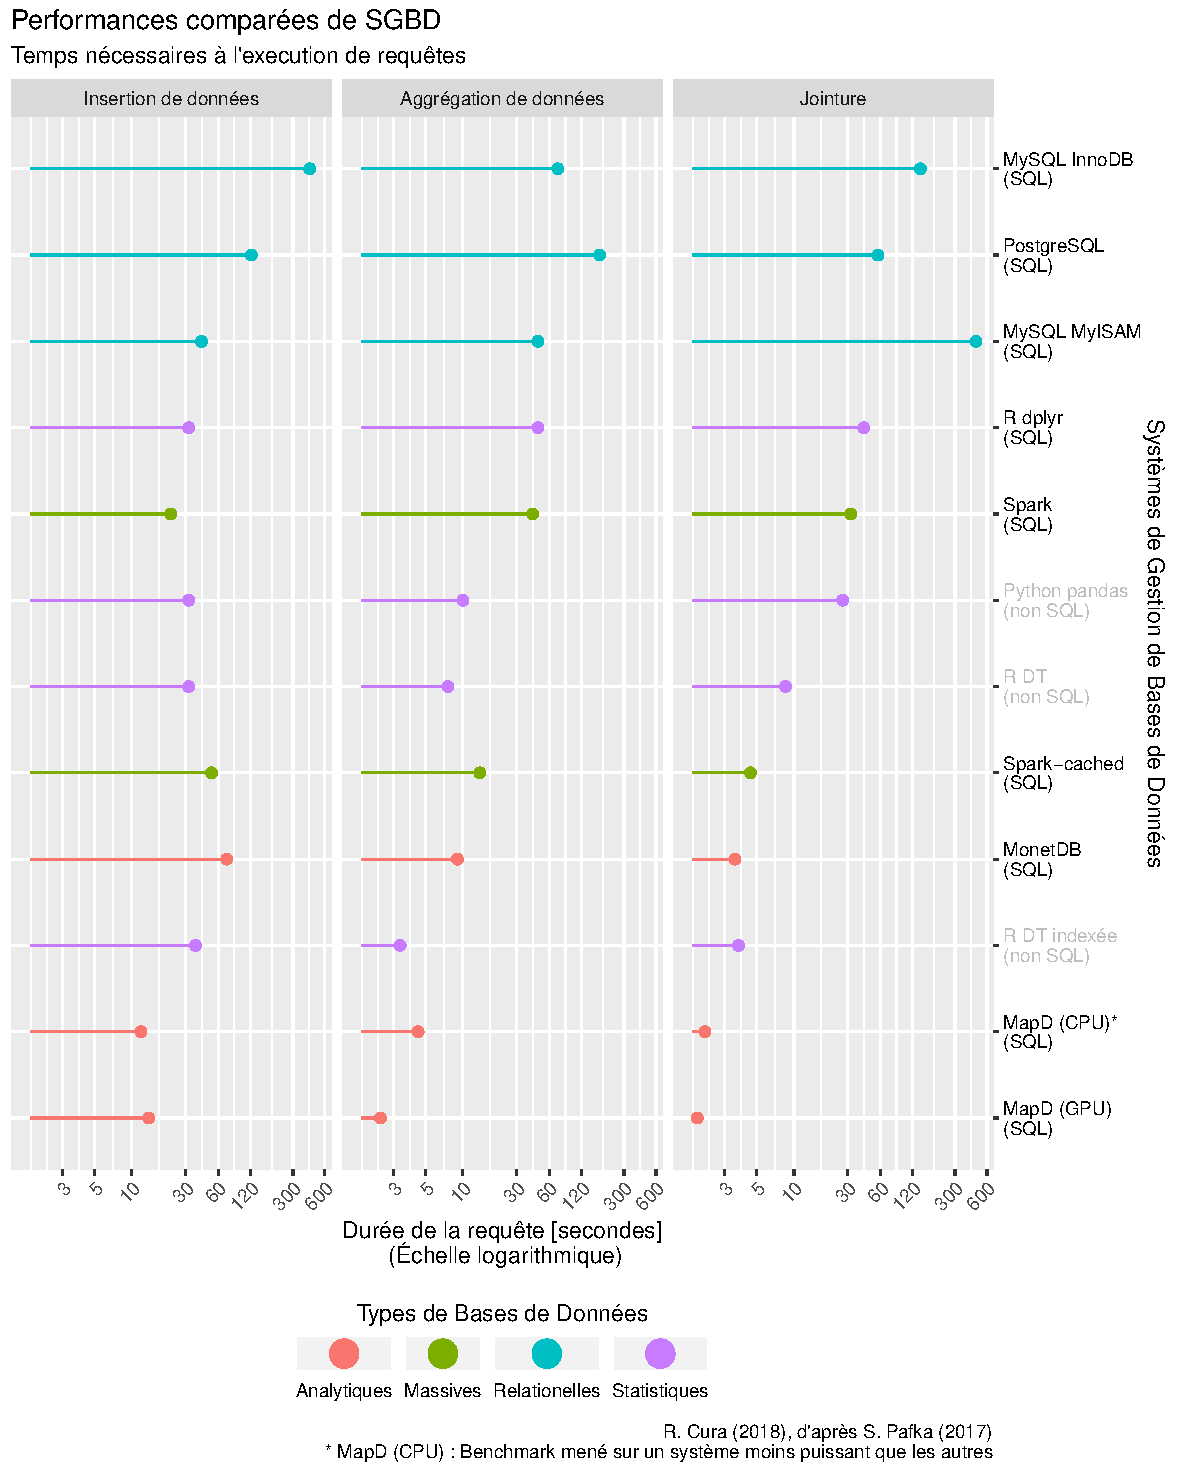
\includegraphics[width=\linewidth]{img/benchmark_results.pdf}
				\caption[Comparaison de la performance de différents SGBD sur un jeu de données test de 100 millions de lignes.]{Comparaison de la performance de différents SGBD sur un jeu de données test de 100 millions de lignes.\\
				Résultats extraits de \autocite{pafka_benchm-databases_2017} enrichis (SQLite, MapD CPU).\\
				Les \og types de Bases de Données\fg{} correspondent aux usages les plus fréquents des SGBD comparés :\\
				- Analytiques : SGBD optimisés pour les traitements de type agrégation, via une architecture orientée colonne plutôt qu'orientée ligne comme dans les SBGD Relationnels\\
				- Massives : SGBD pensés pour la gestion et l'interrogation de données massives (big data), permettant notamment une parallélisation des requêtes.\\
				- Statistiques : SGBD internes aux environnements de traitement de données statistiques, reposant sur une gestion en mémoire vive. Souvent intégrés d'office dans les environnements décrits (R, Python), ce sont les SGBD les plus simples à mettre en place et à manipuler.
			}
				\label{fig:db-benchmarks}
			\end{figure}


			\subparagraph{Performances en écriture et en lecture}

			La \cref{fig:db-benchmarks} affiche des résultats qui semblent globalement ordonnés (les quatre premiers SGBD sont par exemple quasiment toujours plus lents que les 2 derniers), mais fluctuent cependant à la marge selon les opérations demandées.
			La première colonne du graphique montre ainsi le temps nécessaire à l'insertion du jeu de données exemple (100 millions de lignes) dans le SGBD depuis un fichier CSV.
			Les deux colonnes suivants exposent le temps nécessaire au traitement d'une requête, donc à une interrogation des données une fois archivées dans les bases de données.
			On peut constater que le classement des SGBD varie à la marge, et en particulier entre les opération de lecture et d'insertion.
			Dans un environnement classique, la performance d'insertion de données est un facteur prépondérant : quand de nouvelles données sont ajoutées constamment, par exemple pour stocker des données issues de capteurs automatiques, l'insertion peut vite constituer le goulot d'étranglement de la solution.

			Pour SimFeodal, l'insertion n'est pas véritablement un enjeu : les données sont ajoutées par bloc, manuellement, une fois que des nouvelles simulations ont été exécutées.
			C'est donc au pire un acte quotidien, mais dans ce cas, que la requête demande 10 secondes (MapD) ou 10 minutes (MySQL InnoDB), cela n'a que peu d'impact.

			La première colonne donne donc une idée des performances, mais ne revêt pas un critère indispensable dans notre cas.

			Les deux colonnes suivantes, relatives à l'interrogation de données, se révèlent au contraire extrêmement importantes : à chaque action de l'utilisateur de SimEDB, une nouvelle requête est envoyée pour calculer un nouvel indicateur correspondant au jeu de données filtré manuellement (cf. \cref{subsec:explo-interactive}).
			À chaque affichage d'onglet, une nouvelle requête est donc émise et traitée. Même si tous les indicateurs ne sont pas systématiquement mobilisés -- et donc calculés -- (cf. \hl{chap 3}), cela signifie tout de même que pour chaque sélection, une bonne dizaine d'indicateurs seront observés, et donc, autant de requêtes.
			Avec un temps d'exécution de 60 secondes (PostgreSQL en \og jointure\fg{}), cela implique que chaque indicateur requiert une minute avant de s'afficher, et donc, une bonne dizaine de minutes ne serait-ce que pour charger les indicateurs, sans donc tenir compte de la durée nécessaire à leur analyse par l'utilisateur.
			Pour noircir le trait, notons de plus que les résultats communiqués dans la \cref{fig:db-benchmarks} correspondent à des requêtes exemples simples.
			Dans le cas de SimEDB, le calcul des indicateurs requiert des requêtes plus complexes, faisant appel à des agrégations et à des jointures en même temps, et les délais affichés dans ce \textit{benchmark} sont donc bien moindre que les durées éprouvées en conditions réelles au sein de SimEDB.

			\subparagraph{De l'intérêt de gagner quelques secondes}

			La \cref{fig:db-benchmarks} permet d'isoler un sous-ensemble de SGBD ayant, avec le jeu de données testé, des réponses inférieures à une dizaine de secondes.
			On pourrait se contenter de choisir le SGBD le plus complet parmi les 4 solutions identifiées (Spark avec cache, MonetDB ou les deux configurations de MapD).

			Pourtant, les conclusions d'un domaine parallèle se révèlent précieuses pour ne pas suivre ce raisonnement :
			dans le monde des sites internet, donc d'environnements dotés de multiples pages qu'un utilisateur consulte avant de passer à la suivante, de nombreuses études ont montré que la durée d'affichage d'une page jouait de manière considérable sur l'usage d'un site.
			Neil Patel, par exemple, relate une expérience vécue au sein du moteur de recherche Google  :

			\begin{quotation}
				\og
			Google did an interesting experiment with regard to load times. Google Vice President Marissa Mayer asked web surfers – would you rather see 10 or 30 results for your Google search? The users agreed that 30 results per page sounded like a good idea. So Google implemented it on some results pages.\\
			Then the shock came.\\
			Pages that displayed 30 results each had traffic to them drop an astounding 20\%. Google tested the loading difference between the 10 and 30 results pages and found that it was just \textbf{half of a second}. If half of a second made that much of a difference in how long users were willing to wait, how much of a difference could it make to your site if you carved a second or two off of load time?
				\fg{}\\
				\mbox{}~ \hfill  \autocite{patel_speed_2011}
			\end{quotation}

			Si l'environnement et les conditions décrites ne sont naturellement pas directement comparables avec celles de SimEDB, il demeure qu'une différence même faible dans un temps de chargement, ou, pour SimEDB, dans un temps d'affichage d'un indicateur de sortie, pourrait avoir des conséquences négatives pour l'utilisation de la plate-forme.

			Dans un cadre plus proche du notre, relatif au nombre de pages visitées en moyenne sur un site web (\cref{fig:page-abandon}), ce que l'on peut donc directement assimiler au nombre d'indicateurs consultés dans SimEDB, on peut aussi se rendre compte que quelques secondes de différence ont un impact là encore crucial dans l'utilisation qui sera faite d'un site.

			\begin{figure}[H]
				\centering
				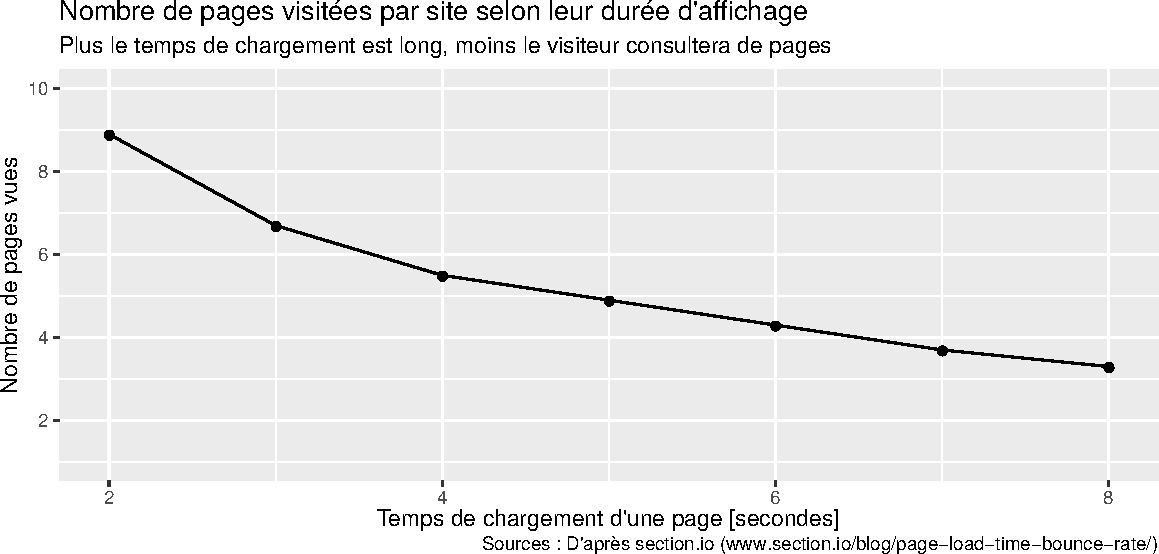
\includegraphics[width=\linewidth]{img/abandon_pages.pdf}
				\caption{Impact du temps de chargement des pages web sur le nombre de pages consultées au cours d'une session. D'après \cite{elliott_how_2017}.}
				\label{fig:page-abandon}
			\end{figure}

			On peut toutefois pondérer ces comparaisons et minimiser l'importance d'écarts de l'ordre de grandeur de la seconde.
			En effet, dans le cas de SimEDB, contrairement à celui d'un site web ou d'un moteur de recherche, l'utilisateur est captif : un thématicien souhaitant explorer les résultats de sur SimFeodal n'aura d'autre choix que de passer par SimEDB.
			De même, sachant que la plate-forme présente pour lui un intérêt professionnel, il sera bien pus patient que face à un quelconque site de courses en lignes.

			Dans le cadre d'environnements de type \textit{visual analysis}, il a été montré que les utilisateurs d'environnement d'exploration étaient toutefois fortement affectés par l'accroissement de délais.
			Zhicheng Liu et Jeffrey Heer \autocite{liu_effects_2014} montrent ainsi qu'en introduisant une latence supplémentaire de 500 ms dans une application interactive d'exploration de données spatio-temporelles, le nombre d'interactions chute fortement, quand bien certains utilisateurs de cette application ne remarquent même pas la différence de délai.

			\paragraph*{}

			Il ressort de cet ensemble successif de filtres que les solutions appropriées à l'organisation des données issues de SimFeodal sont assez peu nombreuses et diverses.
			Au regard des performances de chacun des SGBD, MapD \autocite{root_mapd_2016} présente l'avantage indéniable de la vitesse de traitement des requêtes, tout en étant compatible avec les standards de l'interrogation de données (langage de requête SQL, interfaçable via JDBC).
			Quand bien même nous ne disposons pas des infrastructures qui sont en mesure d'exprimer les meilleurs performances de ce SGBD\footnote{
				MapD est ainsi un SGBD optimisé pour l'analyse sur processeurs graphiques (les GPU), présents dans les cartes graphiques modernes, contrairement aux SGBD classiques qui s'appuient sur les processeurs (CPU) pour effectuer leurs calculs.
			}, MapD est incontestablement plus performant que les autres SGBD, même \og bridé\fg{} -- au sein d'un environnement technique à base de CPU.
			Notons tout de même que le SGBD MonetDB \autocite{vermeij_monetdb_2008}, dans son implémentation intégrée MonetDBLite \autocite{raasveldt_monetdblite_2018}, affiche aussi des performances très compétitives, et aurait pu être choisi pour SimEDB, présentant notamment l'avantage d'être plus utilisé et ancien\footnote{
				Et dans les faits, MonetDBLite a été le SGBD utilisé pendant une large partie de la conception de SimEDB.
				À cette époque, il s'est toutefois révélé assez instable, faisant preuves à plusieurs reprises de corruptions de données ayant entraîné l'obligation de recréer entièrement les bases de données depuis les fichiers bruts produits par SimFeodal.
			}.
		Un des ouvrages de référence en \textit{visual analytics} s'interrogeait d'ailleurs sur les nouvelles possibilités et l'adéquation offertes par ce SGBD (\cite[105]{fekete_infrastructure_2010} in \cite{keim_mastering_2010}).
		Nous avons toutefois préféré MapD, en particulier parce que les données issues de SimFeodal sont amenées à augmenter, renforçant donc petit à petit l'écart de performance entre MapD et MonetDB.
		Par ailleurs, par une heureuse coïncidence, MapD a été placé sous licence libre peu avant que nous n'ayons à nous pencher réellement sur les problèmes de performances et de robustesse qui apparaissaient suite à l'augmentation du nombre de simulations effectuées.


	\subsection{Structuration des données de SimFeodal}

	Une fois le SGBD destiné à stocker les données en sortie de SimFeodal, encore faut-il choisir la manière de les organiser.
	On en peut ainsi pas travailler directement avec les données générées par SimFeodal.

	\paragraph*{Pré-traitement des données}
	Ces données sont des données \og brutes\fg{}, c'est-à-dire qu'elles ne sont pas organisées de manière rationnelle, contiennent une quantité non négligeable d'informations incomplètes et/ou superflues.
	Par exemple, quand une simulation est arrêtée en cours, soit volontairement, soit en raison d'un \textit{bug}, les données des pas de temps réalisés sont tout de même exportées dans les fichiers bruts.
	De la même manière, il arrive qu'on reproduise trop de fois des simulations avec le même jeu de valeurs de paramètres, amenant alors un nombre de réplications supérieur à celui d'autres expériences.
	On peut enfin voir subvenir des erreurs dans les agents, par exemple quand, en raison d'un bug, un agent en interroge un autre qui a disparu depuis.
	Il arrive ainsi fréquemment que des foyers paysans déclarent une appartenance à un agrégat qui a disparu depuis.
	Dans ces cas, fautifs, les données seront aussi inscrites dans les sorties de SimFeodal, quand bien même elles n'ont pas de sens.

	Les données brutes doivent donc nécessairement être vérifiées, filtrées, nettoyées et retravaillées avant de pouvoir les exploiter en vue de générer les indicateurs de sortie.

	\paragraph*{Organisation des données}
	Même pré-traitées, les données brutes conservent une structure tabulaire assez peu adaptées à un traitement : chaque type d'agent stocke ses données correspondantes dans un fichier spécifique, et le nettoyage de celui-ci ne change rien au fait qu'il demeure isolé des autres fichiers.
	Une partie des indicateurs repose sur des analyses croisant différents types d'agents (dans quels pôles les agrégats s'inscrivent-ils par exemple ?), et il est donc nécessaire de permettre -- et de fluidifier -- ces requêtes croisées.
	On a mentionné le choix de SGBD relationnels, il convient donc de concevoir et d'implémenter, dans le SGBD choisi, les relations entre les différentes tables individuelles qui proviennent des sorties brutes de SimFeodal.



		\subsubsection{Quel modèle de données ?}
			\paragraph*{Un modèle \og en étoile\fg{}}

		Là aussi, de nombreuses possibilités existent, autour des schémas traditionnellement utilisés avec des SGBD relationnels.
		Sans entrer dans le détail, notons que chacun des schémas existant présente des avantages et inconvénients liés aux types de requêtes qui lui seront adressés.
		Par exemple, un schéma \og en étoile\fg{}(\textit{star schema}, \autocite{noauthor_star_2018}) privilégie l'efficacité de requêtes d'agrégations et de jointures, au détriment de la robustesse des données et de la liberté des requêtes.
		Au contraire, un schéma \og en flocons\fg{} (\textit{snowflake schema}, \autocite{noauthor_snowflake_2018}) peut se révéler plus permissif en terme de capacités de requêtes, mais au coût d'une plus grande complexité des requêtes de bases.
		Pour choisir un schéma, et donc une manière d'organiser la base de données, il convient donc de savoir -- ou de prévoir -- le type de requêtes qui lui seront adressées.
		Dans le cas des données de SimFeodal, les indicateurs ayant été définis avant que le besoin d'interrogation performante n'apparaisse, on connaissait déjà les indicateurs nécessaires, et donc le type de requêtes qui seraient nécessaires pour les calculer depuis les données brutes issues des simulations.

		Nous savions ainsi qu'une majorité des requêtes seraient des tâches d'agrégations simples (nombre d'agrégats au cours du temps, taux de foyers paysans dispersés au cours du temps etc.), pour lesquelles il fallait donc minimiser la complexité des requêtes et calculs.

		Il a donc été choisi de partir d'un schéma en étoile, puisque celui-ci se montre extrêmement efficace pour réduire les besoins en jointures -- chronophages -- et pour des tâches d'agrégations lourdes.

		Au centre de cette étoile (voir \cref{fig:MCD_SimEDB}), il était donc évident de disposer une table simple, contenant les informations sur lesquelles une majorité des agrégations seraient effectuées : les simulations, identifiées par leur nom (\texttt{sim\_name}, qui permet de savoir de quelle expérience ces simulations dépendent) et leur identifiant unique, la graine aléatoire utilisée (\texttt{seed}).

		\paragraph*{Relier les tables}

		Toutes les tables contenant les enregistrements individuels des agents (\texttt{fp}, \texttt{agregats} etc.) sont donc liées directement à cette table centrale (intitulée \texttt{seeds} ici).

		En dehors de ces tables liées aux agents, deux autres tables \og globales\fg{} sont présentes : une table \og \texttt{results}\fg{}, qui contient des informations agrégées sur l'état de chaque simulation à chaque pas de temps. Ces informations, par exemple le taux de foyers paysans isolés (champ \og \texttt{prop\_fp\_isoles}\fg{}), sont redondantes : elles pourraient être calculées directement depuis la table renseignant les foyers paysans, en faisant un ratio entre le nombre de foyers paysans sans agrégat et leur nombre total.
		Pourtant, pour des raisons d'efficacité autant que de clarté, il a été choisi de dupliquer, en les pré-calculant, ces informations qui sont interrogées extrêmement souvent pour calculer les indicateurs de SimFeodal.

		L'autre table ne répondant pas au schéma classique est la table \og \texttt{parameters}\fg{}, qui fournit toutes les méta-données sur les simulations. On y retrouve par exemple les valeurs de paramètres de chacune des simulations, identifiées toujours par le couple \texttt{sim\_name} et \texttt{seed}.
		Cette table est la seule à être reliée bi-directionnellement à la table centrale (\texttt{seeds}), en particulier en raison de l'usage qui en est fait interactivement (voir la \cref{fig:MCD_SimEDB_etapes}).

		Notons tout de même que l'on s'éloigne légèrement du classique schéma en étoile en raison des relations que nous avons choisi d'insérer entre les tables des différents agents (relations notées en pointillées dans la \cref{fig:MCD_SimEDB}).
		Intégrer ces relations dans la table centrale aurait considérablement complexifié cette dernière, mais pour autant, elles étaient nécessaires : SimFeodal est un modèle complexe, dans lequel des interactions sont présentes à plusieurs niveaux entre différents types d'agents. La base de données résultant de ce modèle complexe l'est donc nécessairement aussi, et ne peut s'épargner de relations entre les agents correspondant aux interactions éprouvées.
		Ici, ces relations permettent par exemple d'étudier la composition des pôles autour de chaque agrégat, et ainsi d'étudier le lien entre poids du pôle (en nombre d'attracteurs) et poids de l'agrégat (en nombre de foyers paysans).

		Ce type d'indicateur est toutefois moins utilisé que les indicateurs plus directs (\hl{ref à chapitre 3, indicateurs}), et les requêtes correspondantes, moins fréquentes, ne perturbent pas les logiques et performances d'ensemble de SimEDB.

\clearpage
		\begin{figure}[H]
			\centering
			\captionsetup{width=\linewidth}
			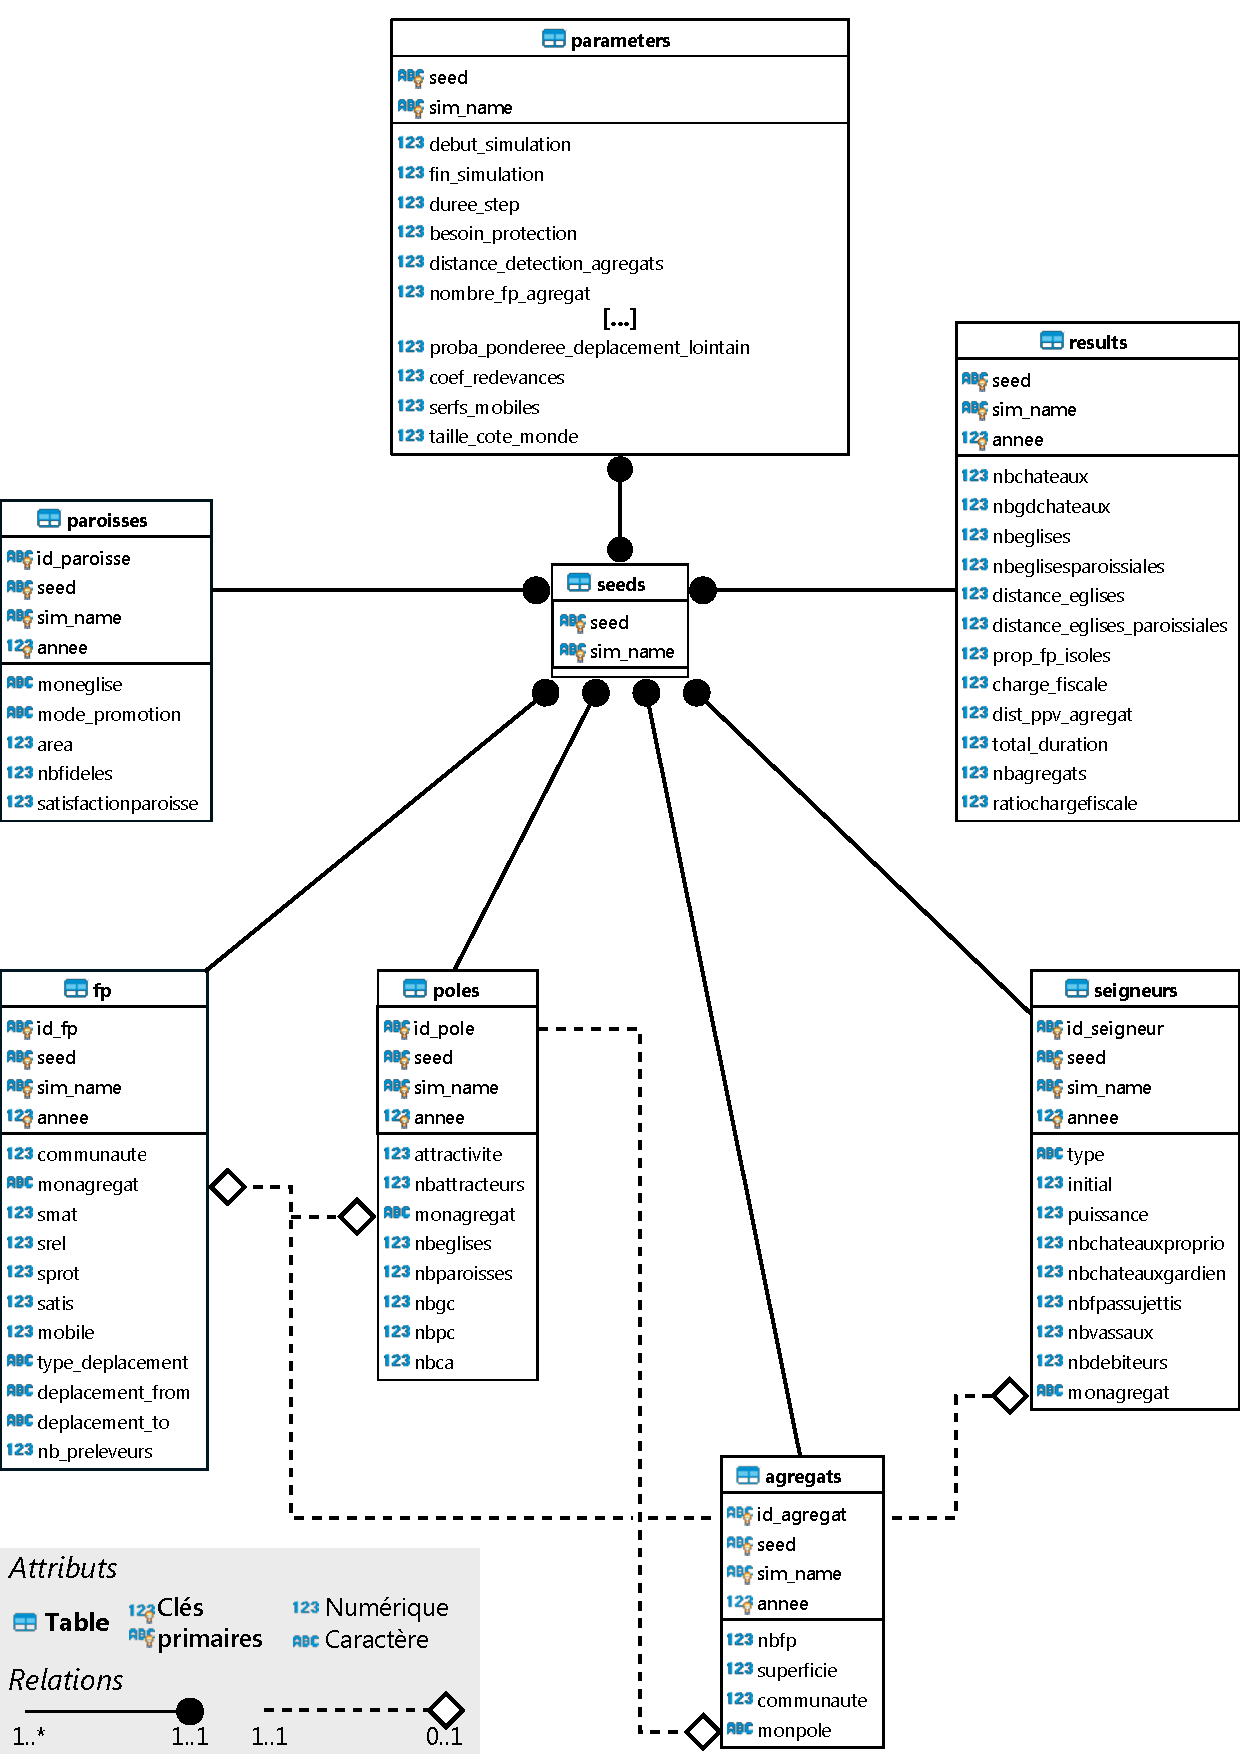
\includegraphics[width=\linewidth]{img/MCD_SimEDB_repris.pdf}
			\caption{Modèle Conceptuel de Données (MCD) des données en sortie de simulation de SimFeodal telles qu'implémentées dans SimEDB.}
			\label{fig:MCD_SimEDB}
		\end{figure}
\clearpage

\begin{figure}[H]
	\centering
	\captionsetup{width=\linewidth}
	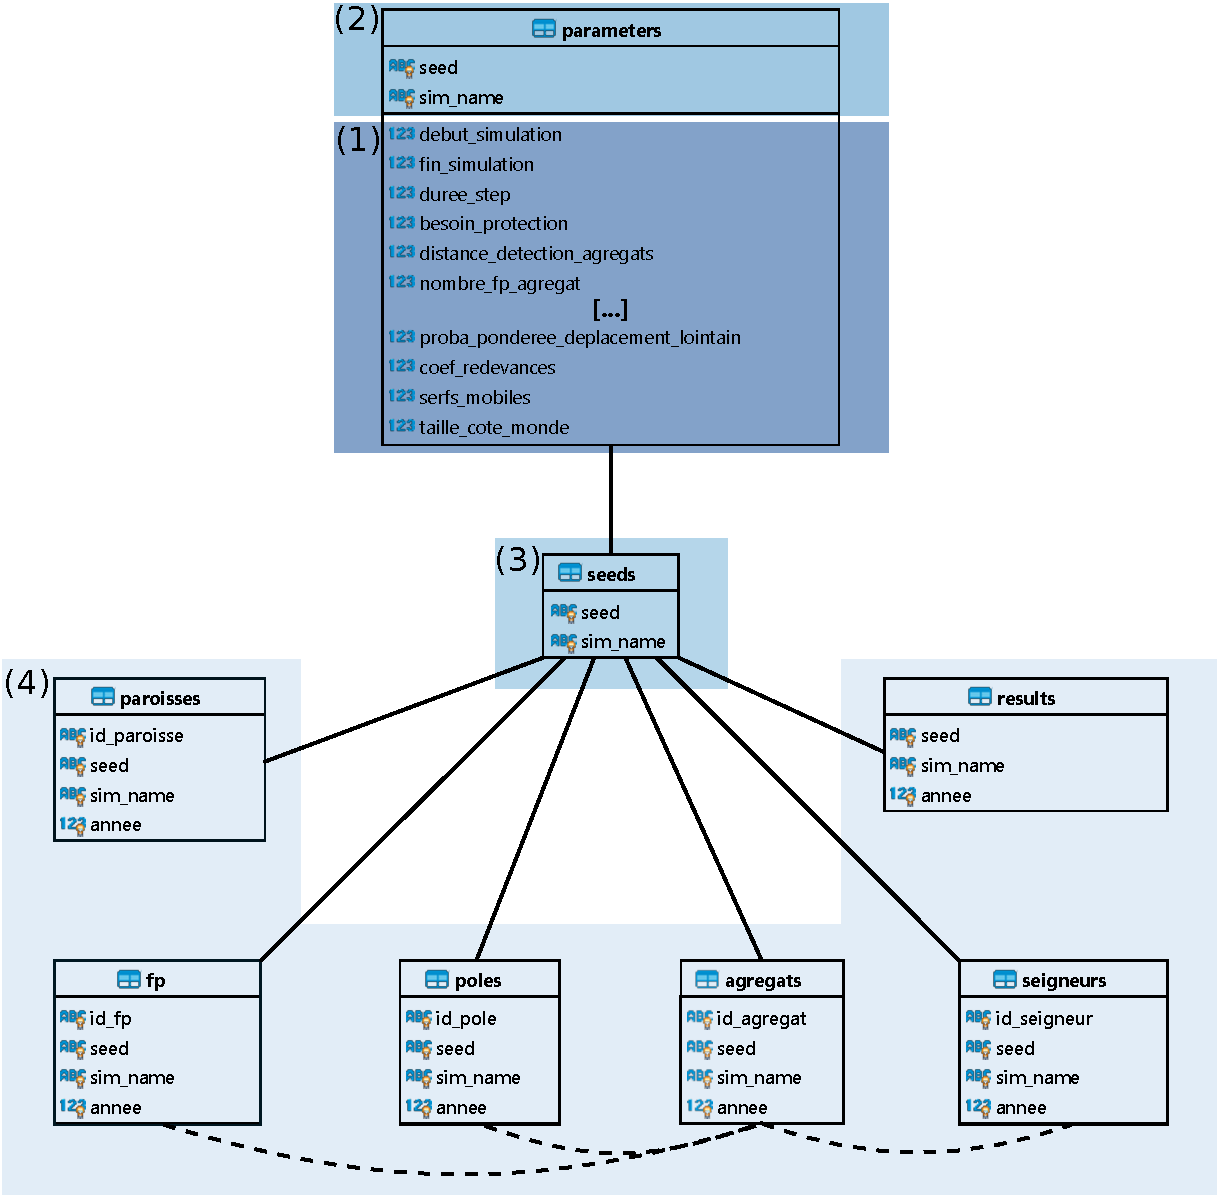
\includegraphics[width=\linewidth]{img/MCD_SimEDB_simplified.pdf}
	\caption{Les étapes d'interrogation de la BDD de SimEDB :\\
		(1) Filtrage d'un sous-ensemble de valeurs de paramètres ;
		(2) Les simulations associées sont isolées dans la table des paramètres;
		(3) Répercussion de ce filtre dans la table contenant les identifiants des simulations ;
		(4) Toutes les tables sont filtrées en répercussion}
	\label{fig:MCD_SimEDB_etapes}
\end{figure}
\clearpage
		\subsubsection{Un modèle de données pour favoriser l'interrogation et le filtrage conjoint}

		Le schéma choisit, et le Modèle Conceptuel de Données (MCD) associé, permettent donc une interrogation rapide des données en simplifiant les tâches d'agrégation et en minimisant la quantité de jointures nécessaires à la génération des indicateurs de sortie.

		Le choix de s'écarter légèrement du schéma en étoile présente un autre avantage, extrêmement utile, dans le cadre d'une exploration interactive des indicateurs de SimFeodal.
		En effet, comme on l'a vu auparavant (\cref{subsec:explorer-simedb}), dans SimEDB, on compare les simulations en les isolant à partir des valeurs de paramètres qui leur correspondent, via un acte de \textit{brushing} des valeurs de paramètres présentées dans un graphique en coordonnées parallèles interactif.

		Du côté du MCD, la table correspondante est la table \texttt{parameters}. Quand l'utilisateur sélectionne un sous-ensemble de valeurs de paramètres, la table est filtrée, et ne renvoi donc que les simulations correspondantes.

		C'est ici que l'intérêt de la table \texttt{seeds} et de son lien bidirectionnel avec la table \texttt{parameters} apparaît : une fois \texttt{parameters} filtrée, cette sélection est renvoyée à la table \texttt{seeds}, et se répercute donc directement à toutes les autres tables.
		Avec une unique requête, qui plus est sur une table de faible dimension (\texttt{seeds} ne comporte que deux champs), le filtrage est donc extrêmement véloce, accélérant d'autant le filtrage des autres tables et donc la génération des indicateurs de sortie.

		Ces étapes de filtrage successifs, optimisées par l'architecture choisie pour les données de SimFeodal, sont schématisées dans la \cref{fig:MCD_SimEDB_etapes}.


		\subsection*{Une organisation dédiée à l'exploration interactive}
		La présentation des choix d'organisation de données témoigne d'une visée résolument applicative, c'est-à-dire visant à penser l'organisation, la structuration et les SGBD d'implémentation, comme au service de la plate-forme d'exploration SimEDB.
		Le SGBD choisi, MapD, est ainsi un logiciel particulièrement adapté aux besoins identifiés, c'est-à-dire à une efficacité et une robustesse d'interrogation des données générées par SimFeodal.
		MapD est interrogeable de manière universelle, via des protocoles de connexion standards, au moyen d'un langage qui fait office de \textit{lingua franca} de l'interrogation de données, le SQL.
		Au sein du SGBD, la structure des données, révélée dans le MCD qui adopte une structure \og en étoile\fg{}, vise aussi à faciliter et à optimiser la vitesse des requêtes visant à générer les indicateurs de sortie de SimFeodal.
		Cette structure de données est enfin pensée, en amont, pour minimiser le nombre requêtes nécessaires à l'affichage des indicateurs, dans un cadre interactif, correspondant à des sous-ensembles des nombreuses simulations effectuées au cours de la construction, du paramétrage et de la calibration de SimFeodal.

		Il est important de noter qu'en l'absence de ces choix de conception de base de données, de la modélisation conceptuelle jusqu'à l'implémentation technique, la plate-forme d'exploration des données SimEDB, que nous allons maintenant présenter plus en détail, n'aurait pu être conçue, élaborée et bâtie de manière convaincante.